\documentclass{article}

\usepackage{graphicx}
\usepackage{tikz}
\usepackage{tikzsymbols}
\usetikzlibrary{calc,patterns,shapes.geometric}
\pagestyle{empty}
\usepackage[margin=0pt]{geometry}
\geometry{papersize={14in,12in}}

\def\centerarc[#1](#2)(#3:#4:#5){\draw[#1] ($(#2)+({#5*cos(#3)},{#5*sin(#3)})$) arc (#3:#4:#5);}

\begin{document}
	\begin{figure}
		\centering
		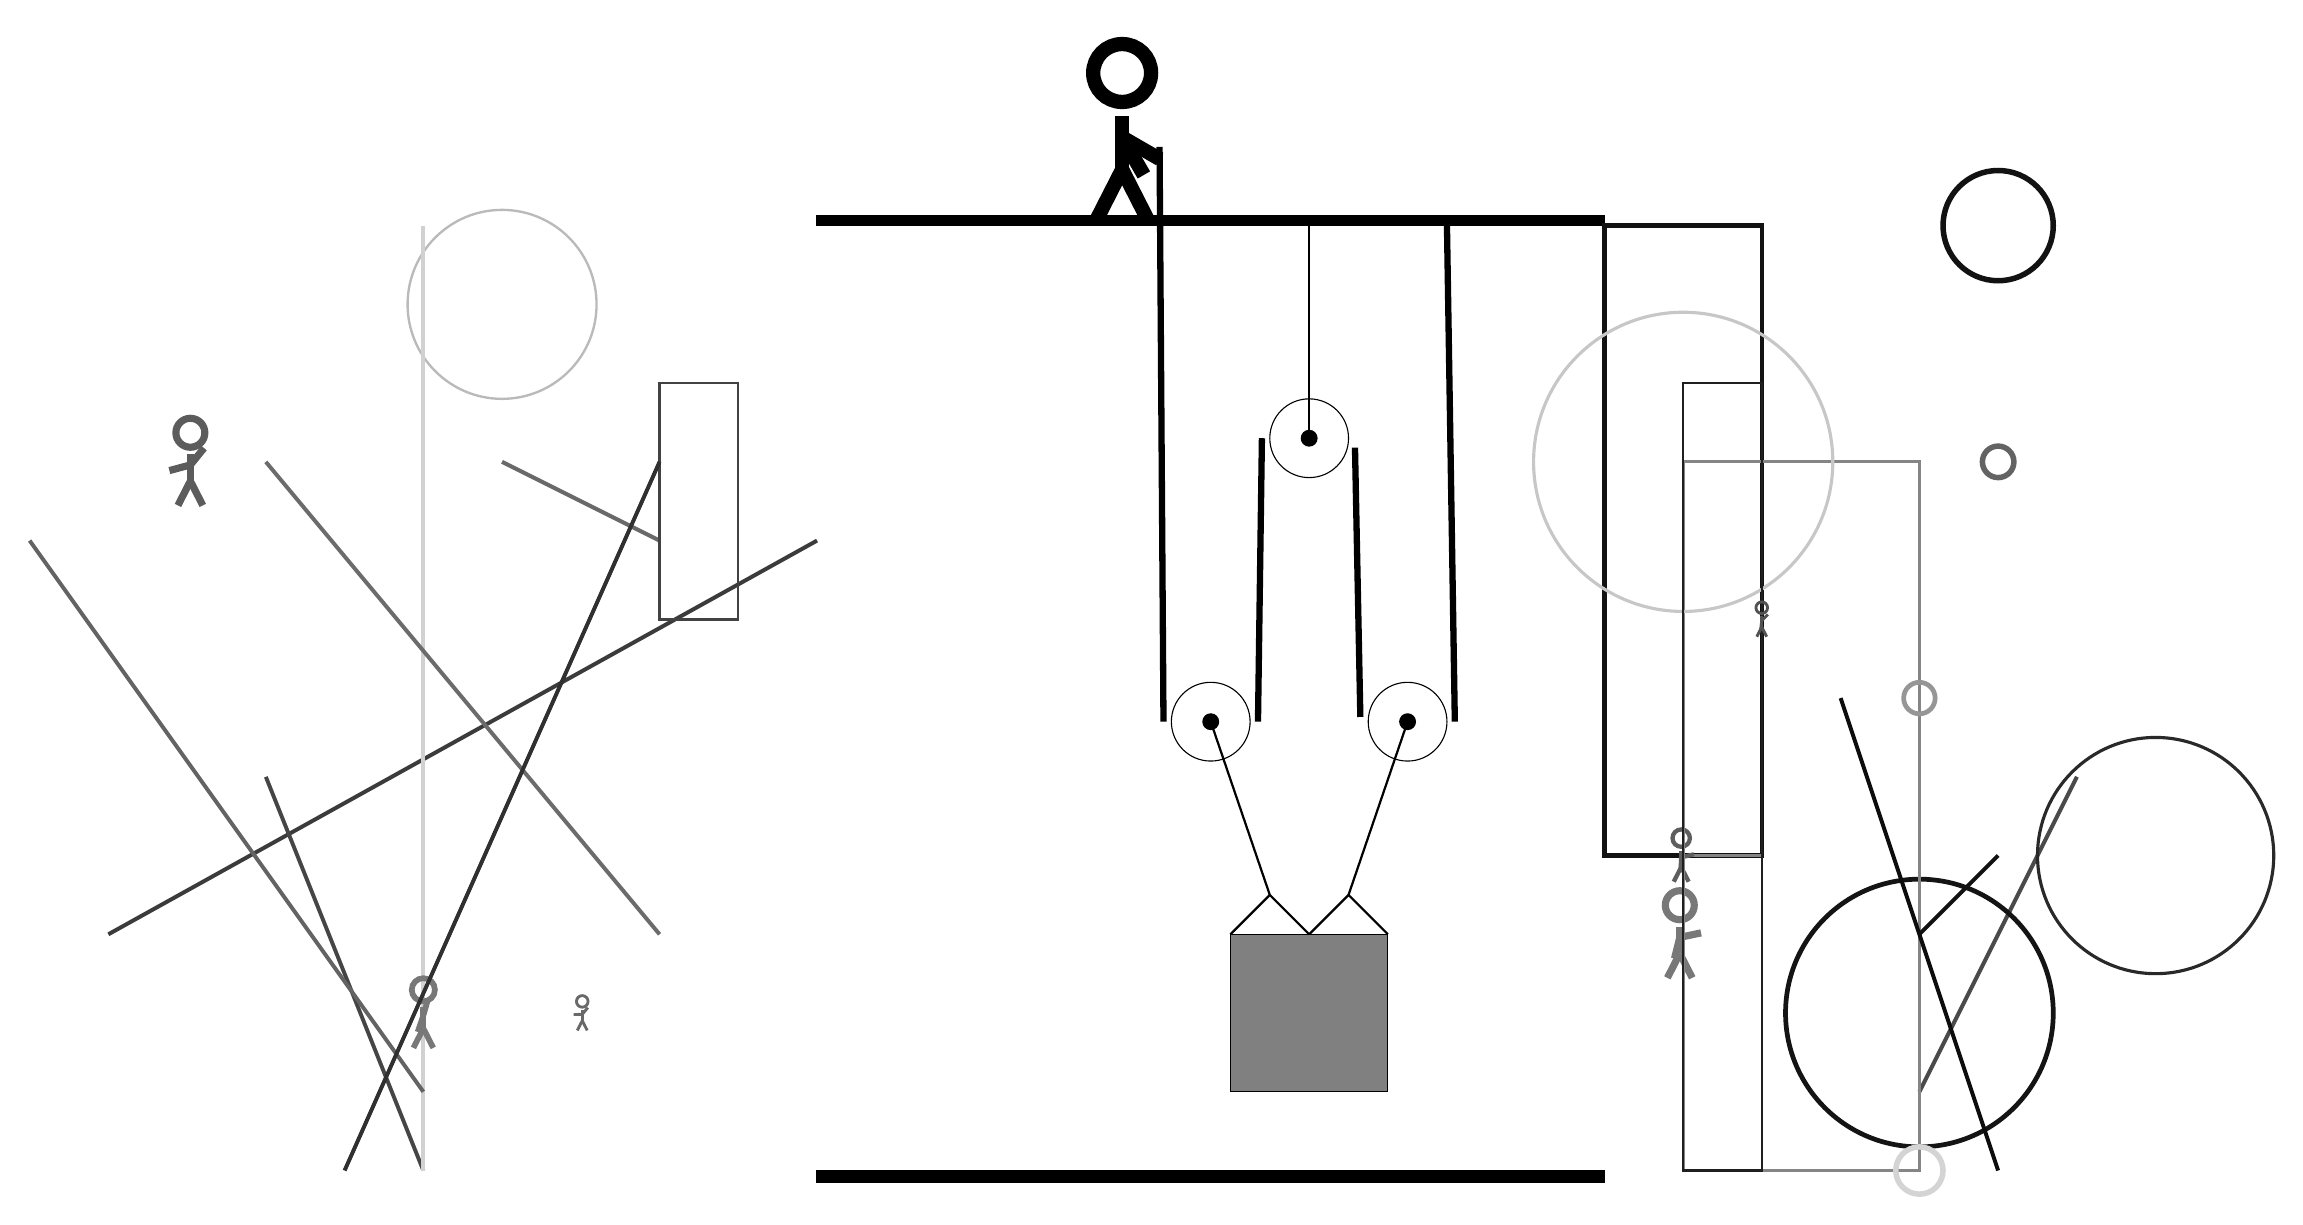
\begin{tikzpicture}
			%%%%% START %%%%%
			
			\draw[fill=black] (-4, 9) rectangle (6, 9.125);
			
			\draw (1, 2.7) circle (0.5);
			\draw[fill=black] (1, 2.7) circle (0.1);
			
			\draw (2.25, 6.3) circle (0.5);
			\draw[fill=black] (2.25, 6.3) circle (0.1);
			\draw[thick] (2.25, 6.3) -- (2.25, 9);
			
			\draw (3.5, 2.7) circle (0.5);
			\draw[fill=black] (3.5, 2.7) circle (0.1);
			
			\draw[thick] (3.5, 2.7) -- (2.75, 0.5);
			\draw[thick] (1, 2.7) -- (1.75, 0.5);
			\draw[thick]  (1.25, 0) -- (1.75, 0.5) -- (2.25, 0);
			\draw[thick]  (2.25, 0) -- (2.75, 0.5) -- (3.25, 0);
			\draw[fill=black!50] (1.25, 0) rectangle (3.25, -2);
			
			\draw[line width=0.5mm, color=black!71](10, -2) -- (12, 2);
			
			\draw[line width=0.6mm, color=black!93] (6, 9) rectangle (8, 1);
			\draw[line width=0.5mm, color=black!77](-4, 5) -- (-13, 0);
			\node[line width=0.4mm, color=black!53] at (7, 0) {\Strichmaxerl[5][76][12]};
			
			\draw[line width=0.3mm, color=black!48] (7, 7) rectangle (8, 1);
			
			\node[line width=0.4mm, color=black!63] at (7, 1) {\Strichmaxerl[3][87][14]};
			\draw [line width=0.4mm, color=black!84](13, 1) circle (1.5);
			
			\draw[line width=0.5mm, color=black!59](-6, 5) -- (-8, 6);
			\node[line width=0.3mm, color=black!59] at (-7, -1) {\Strichmaxerl[2][2][50]};
			\draw [line width=0.7mm, color=black!93](11, 9) circle (0.7);
			\draw [line width=0.6mm, color=black!92](10, -1) circle (1.7);
			\draw[line width=0.4mm, color=black!48] (7, 6) rectangle (10, -3);
			\draw[line width=0.3mm, color=black!74] (-5, 7) rectangle (-6, 4);
			
			\draw[line width=0.5mm, color=black!73](-9, -3) -- (-11, 2);
			\draw [line width=0.3mm, color=black!27](-8, 8) circle (1.2);
			\draw [line width=0.4mm, color=black!22](7, 6) circle (1.9);
			
			\draw[line width=0.5mm, color=black!18](-9, -3) -- (-9, 9);
			\draw[line width=0.3mm, color=black!88] (7, 7) rectangle (8, -3);
			\draw [line width=0.7mm, color=black!61](11, 6) circle (0.2);
			\draw[line width=0.5mm, color=black!93](10, 0) -- (11, 1);
			\draw[line width=0.5mm, color=black!61](-9, -2) -- (-14, 5);
			\node[line width=0.6mm, color=black!53] at (-9, -1) {\Strichmaxerl[4][71][74]};
			\draw [line width=0.6mm, color=black!41](10, 3) circle (0.2);
			\draw[line width=0.5mm, color=black!58](-6, 0) -- (-11, 6);
			\draw [line width=0.7mm, color=black!36](11, 3) circle (0.0);
			
			\node[line width=0.5mm, color=black!68] at (8, 4) {\Strichmaxerl[2][83][45]};
			\draw[line width=0.5mm, color=black!95](11, -3) -- (9, 3);
			\draw [line width=0.7mm, color=black!17](10, -3) circle (0.3);
			\node[line width=0.4mm, color=black!64] at (-12, 6) {\Strichmaxerl[5][15][51]};
			\draw[line width=0.5mm, color=black!81](-6, 6) -- (-10, -3);
			
			\draw[line width=0.8mm] (0.35, 10) --  (0.4, 2.7);
			\centerarc[line width=0.8mm](1, 2.7)(180:360:0.6);
			\draw[line width=0.8mm] (1.6, 2.7) -- (1.65, 6.3);
			\centerarc[line width=0.8mm](2.25, 6.3)(-20:180:0.6);
			\draw[line width=0.8mm](2.832, 6.18) -- (2.9, 2.76);
			\centerarc[line width=0.8mm](3.5, 2.7)(160:360:0.6);
			\draw[line width=0.8mm](4.1, 2.7) -- (4.0, 9);
			
			\node at (-0.07, 10.2) {\Strichmaxerl[10][120][-30]};
			
			\draw[fill=black] (-4, -3) rectangle (6, -3.15);
			
			%%%%% END %%%%%
		\end{tikzpicture}
	\end{figure}	
\end{document}